\documentclass{sig-alternate-05-2015}
\usepackage{graphicx}
\usepackage{amsfonts}
\usepackage{amssymb}
\usepackage{textcomp}
\usepackage{subfig}
\begin{document}
% Copyright
\setcopyright{acmcopyright}
%\setcopyright{acmlicensed}
%\setcopyright{rightsretained}
%\setcopyright{usgov}
%\setcopyright{usgovmixed}\usepackage{amsmath}


%\setcopyright{cagov}
%\setcopyright{cagovmixed}


% DOI
\doi{10.475/123_4}

% ISBN
\isbn{123-4567-24-567/08/06}

%Conference
\conferenceinfo{PLDI '13}{June 16--19, 2013, Seattle, WA, USA}

\acmPrice{\$15.00}

%
% --- Author Metadata here ---
\conferenceinfo{WOODSTOCK}{'97 El Paso, Texas USA}
%\CopyrightYear{2007} % Allows default copyright year (20XX) to be over-ridden - IF NEED BE.
%\crdata{0-12345-67-8/90/01}  % Allows default copyright data (0-89791-88-6/97/05) to be over-ridden - IF NEED BE.
% --- End of Author Metadata ---

\title{Performance Analysis of TCP Variants}

%
% You need the command \numberofauthors to handle the 'placement
% and alignment' of the authors beneath the title.
%
% For aesthetic reasons, we recommend 'three authors at a time'
% i.e. three 'name/affiliation blocks' be placed beneath the title.
%
% NOTE: You are NOT restricted in how many 'rows' of
% "name/affiliations" may appear. We just ask that you restrict
% the number of 'columns' to three.
%
% Because of the available 'opening page real-estate'
% we ask you to refrain from putting more than six authors
% (two rows with three columns) beneath the article title.
% More than six makes the first-page appear very cluttered indeed.
%
% Use the \alignauthor commands to handle the names
% and affiliations for an 'aesthetic maximum' of six authors.
% Add names, affiliations, addresses for
% the seventh etc. author(s) as the argument for the
% \additionalauthors command.
% These 'additional authors' will be output/set for you
% without further effort on your part as the last section in
% the body of your article BEFORE References or any Appendices.

\numberofauthors{2} 
\author{
\alignauthor
Neeki Hushyar\\
       \affaddr{UMass Amherst}\\
       \email{nhushyar@cs.umass.edu}
% 2nd. author
\alignauthor
Angela Upreti\\
       \affaddr{UMass Amherst}\\
       \email{aupreti@cs.umass.edu}
}
\additionalauthors{Additional authors: John Smith (The Th{\o}rv{\"a}ld Group,
email: {\texttt{jsmith@affiliation.org}}) and Julius P.~Kumquat
(The Kumquat Consortium, email: {\texttt{jpkumquat@consortium.net}}).}
\date{30 July 1999}
% Just remember to make sure that the TOTAL number of authors
% is the number that will appear on the first page PLUS the
% number that will appear in the \additionalauthors section.

\maketitle
\input{abstract}


%
% The code below should be generated by the tool at
% http://dl.acm.org/ccs.cfm
% Please copy and paste the code instead of the example below. 
%
\begin{CCSXML}
<ccs2012>
<concept>
<concept_id>10003033.10003079.10011704</concept_id>
<concept_desc>Networks~Network measurement</concept_desc>
<concept_significance>300</concept_significance>
</concept>
<concept>
<concept_id>10003033.10003083.10003014.10011617</concept_id>
<concept_desc>Networks~Firewalls</concept_desc>
<concept_significance>300</concept_significance>
</concept>
<concept>
<concept_id>10003033.10003068.10003069.10003071</concept_id>
<concept_desc>Networks~Deep packet inspection</concept_desc>
<concept_significance>100</concept_significance>
</concept>
</ccs2012>
\end{CCSXML}


%
% End generated code
%

%
%  Use this command to print the description
%
\printccsdesc

% We no longer use \terms command
%\terms{Theory}

\keywords{TCP variants; Comparison; SACK; Reno; New Reno, Vegas; Tahoe }

 \section{Introduction}\label{sec:introduction}
 Web traffic runs over TCP and given the scale at which the internet has grown and how much we rely on the web, it is important that the underlying transport protocol is able to operate at a reasonably low latency and provide high throughput. Network congestion causes packet loss which increases latency and hence, reduces throughput. Using the right TCP variant saves both money and time. Amazon found that every 100ms latency cost then 1 percent in sales~\cite{kohavi_online_2007}. Higher latency/wait-time in web applications discourages clients from revisiting the cite. This is specially true for video applications such as youtube. Clients usually close the page if the latency is high. Fairness in a the underlying transport layer is equally important. One flow should not hog most of the network bandwidth and throttle other flows. Otherwise, different customers paying the same amount for internet service would get widely different performance. Metrics such as throughput, average and end-to-end latency, packet drop rate, fairness are different across different tcp variants and the congestion control algorithms they use. 

Congestion control algorithm for TCP was proposed by Van Jacobson  in response to 1986's `congestion collapse'. The original TCP proposed by Van Jacobson contained elements such as dynamic window sizing, slow start, additive increase and multiplicative deacrease (AIMD). Since then, several variants of TCP have been proposed. TCP Reno adds fast recovery and fast retransmit to TCP Tahoe. TCP Reno's fast recovery and fast retransmit suffer when multiple packets are dropped from the same window. In presence of multiple packet loss, the TCP pipe often gets drained. NewReno has to wait for retransmit timeout to be able to send data again. Consequently, multiple packet loss leads to low throughput. TCP NewReno was introduced to solve this. When in fast recovery, TCP NewReno interprets a single partial Ack as a signal to retransmit another packet rather. NewReno does not wait for 3 duplicate ACKs before retransmitting. TCP SACK is another TCP variant that solves the multiple packet drop problem in Reno. SACK allows the receiver to acknowledge any non sequential packets it has received. NewReno  without SACK is unable to tell exactly which packets are missing. While NewReno can retransmit only one lost packet per RTT, TCP SACK can transmit as many lost packets as the congestion window allows. Variant Vegas uses RTT as an estimate of congestion rather than using packet loss.\\

 We conduct three different simulation studies in this paper:
 \begin{enumerate}
 \item Compare performances of Tahoe, Reno, NewReno, and Vegas under congestion. 
 \item Compare fairness between different TCP variants.
 \item Study influence of queuing disciplines (1)RED and (2) Drop Tail on TCP Sack and TCP Reno.
 \end{enumerate}
 
 

 \section{Methodology}\label{sec:methodology}
  \subsection{The Setup}
  \begin{figure}[!htbp]
  	\centering 
	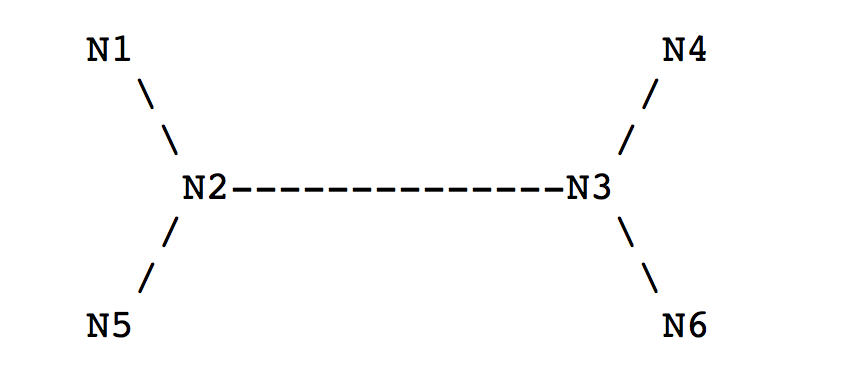
\includegraphics[scale=0.4]{setup.png}
	\caption{We attach TCP agent with FTP as the application, UDP with CBR to this topology.}
	\label{fig:setup}
\end{figure}
We use ns2 to create the topology in Figure \ref{fig:setup}. The setup consists of five different nodes, N1- N5. The link between each pair of nodes is a duplex link with a capacity of 10 Mb.
\subsection{Calculation}
NS2 trace files were used to calculate drop rate, average throughput, average latency and latency over time for combinations of different TCP variants and different queuing algorithms. The trace files were parsed using a python script because of the ease of text parsing with python. We used a python library called the Matplotlib to generate the plots. We use a bash script to automate a series of experiments with varying TCP variant, CBR rate, CBR packet size and queuing algorithms. 
\begin{enumerate}
\item \textbf{Average Throughput:} To calculate the average throughput of the tcp stream, we divide the sum of packet sizes of all TCP packets that reached the destination by the  total time of the tcp flow. 
\item \textbf{Latency:} To calculate latency over time, we recorded the time it took for each packet to get from the source to desination over time. We took the average of latencies over time to get the average latency. 
\item \textbf{Drop Rate:} The ns trace clearly identified the dropped packets. To calculate the drop rate of a flow, we divided the total number of drops by the total number of packets in that flow.
\end{enumerate}
 \subsection{TCP Performance Under Congestion}
This experiment was designed to test the performance of different TCP variants Tahoe, Reno, NewReno and Vegas under various levels of congestion. TCP agent was attached to start at N1 and sink at N4. FTP application was attached to the TCP agent to simulate traffic that is typical of FTP. CBR flow was added to go from N2 to N3 to create congestion in the link between N2 and N3. We varied the CBR rate from 1 Mbps to 10 Mbps to create different levels of congestion. We had the liberty of choosing the packet size to maintain the CBR. To study the effects of varying CBR packet sizes, we also simulated varying packet sizes, 500B to 10,000B, for all four TCP variants. We did not change the default ns2 buffer size of 20 packets.  
 \subsection{Fairness between TCP variants}
This experiment simulated two TCP flows at a time. The variant pairs that were simulated are (1) Tahoe/Tahoe (2) Reno/Reno (3) NewReno/Reno (4) Vegas/Vegas (5) NewReno/Vegas. Like before, to create varying levels of congestion, a CBR flow was added to originate at N2 and end at N3. The first TCP stream originated at added N1 and ended at N4. The second TCP stream originated at N5 and ended at N6. For each pair of the variants, we ran simulations for CBR ranging from 1 Mbps to 10 Mbps. The packet size was 500, constant across all the experiments. We chose this packet size because an average IP packet size is around 600. Accounting for the IP headers, we wanted a smaller packet size for UDP. 
We also started the two competing variants at different times and ran the simulations for a bit longer (15s) to check if fair throughput could be achieved over time if one of the TCP streams was delayed.
 \subsection{Influence of Queuing}
In this experiment, we study the influence of queuing algorithms RED and DropTail on TCP Reno and SACK. The set up for this experiment is the same as experiment 1. We first start the TCP stream, wait till it has passes the slow start phase(at 4s) and then start the CBR flow. We conduct the experiments for two different buffer sizes, 100 and a 300. To compare the performance of RED and DropTail in the TCP variants and the CBR flow, we compare the differences in throughput over time, latency over time and the drop rate between the queuing disciplines. 
\section{Experiment 1: Analyzing Performance of TCP Variants}

This experiment analyzed the performance of different TCP variants over a setup consisting of a single TCP stream and a single CBR flow. The performance of the TCP variants were analyzed over a range of different packet sizes and transmission rates assigned to the CBR. We analyze the results of this experiment in two parts. First, by looking at the performance of the variants over an increasing range of CBR packet sizes, while the rate of the CBR is constant at 2Mbps. Second, we look at the performance of the variants over an increasing range of CBR flows - from 1 Mbps to 10 Mbps, while the size of the initial packet is held constant at 3,000 bytes.

When holding the CBR steady, at 2Mbps, none of the variants experienced any packet loss over the range of increasing packet sizes, from 500 bytes to 8,000 bytes. The average and end-to-end latency as well as the throughput for TCPs  Reno, NewReno and Tahoe were all the same. The throughput hovered around 1 Mbps as the size of packets increased and the average latency hovered around .02 seconds per segment. The average and end-to-end latency of TCP Vegas was slightly smaller, likely because Vegas never saturates the full capacity of the link. Doing so, would imply congestion and the throughput would decrease. The throughput for Vegas hovered at just under .99 Mbps as the size of the packets increased and the latency hovered around .005 seconds.

\begin{figure}[!htbp]
	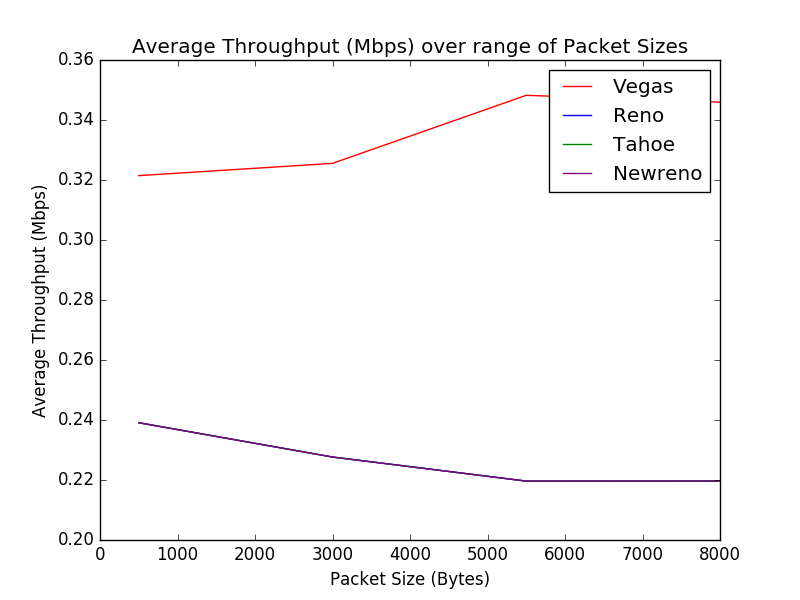
\includegraphics[scale=0.4]{P1.png}
	\caption{This figure plots the average throughput of each TCP variant over a range of CBR flow rates. The packet size is initialized to 3,000 bytes.}
	\label{a:label}
\end{figure}

When the packet size is held steady, at 3,000 bytes and the CBR flow is increased from 1 Mbps to 10 Mbps, all four variants suffer packet loss. Reflected in Figure 3, TCPs Reno, NewReno and Tahoe suffer their first packet drops at a CBR of 7 Mbps. TCP Vegas does not suffer any packet drops, but the throughput is consistently lower than the other variants, as it is reducing its congestion window size to reflect the increasing RTT of the packets. TCP Vegas takes preventative measures to avoid packet loss. The other variants make changes only in the aftermath of packet loss. To prevent congestion, Vegas records the round trip time (RTT) of packets and adjusts its congestion window according to any delay. Our experiments never reached a point at which TCP Vegas experienced packet loss.

\begin{figure}[!htbp]
	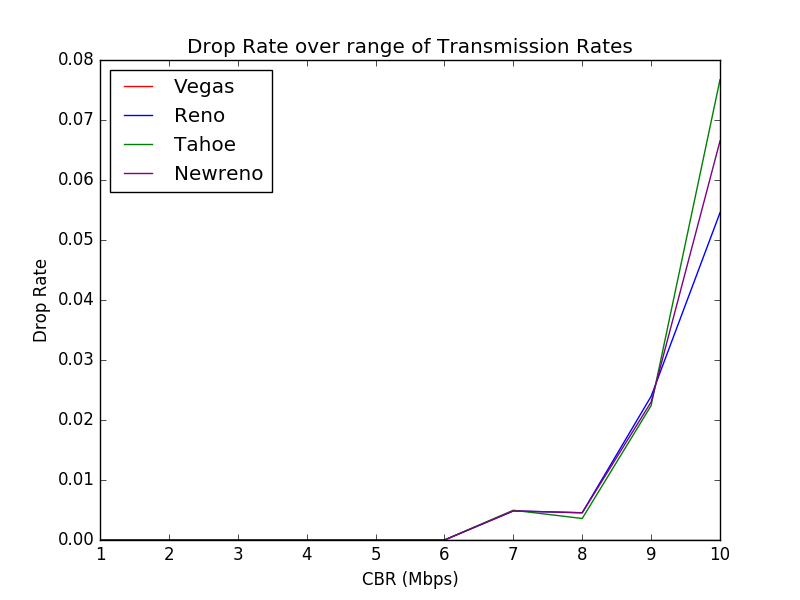
\includegraphics[scale=0.4]{P2.png}
	\caption{This figure plots the number of packets dropped by each TCP variant over a range of CBR flow rates. The packet size is initialized to 3,000 bytes.}
	\label{a:label}
\end{figure}

Each variant is consistent, only in that they wait until receiving 3 duplicate-acknowledgements or retransmit timeouts before retransmitting the first lost packet. 

Given low-to-moderate levels of congestion, TCP Vegas is able to efficiently decrease its congestion window size before experiencing packet loss, and thus is able to maintain zero packet loss while its counterparts are unable to. NewReno, handles multiple packet losses better than Reno and Tahoe. After the first packet loss is identified by a triple duplicate acknowledgement, or by a retransmission timeout, NewReno assumes that any packet following a partial acknowledgment is lost. This makes the retransmission of packets much faster and accounts for the increase in throughput experienced by NewReno in Figure 2.



\section{Experiment 2: Analyzing Fairness between TCP Variants}

This experiment used two TCP flows and a single CBR flow, to analyze the fairness between the TCP flows among different pairs of TCP variants. We tested different combinations of variants, including assigning TCP Vegas to both flows, TCP Reno to both flows, NewReno to one flow and Reno to another, and NewReno to one flow and Vegas to another. Further, we ran two slightly different simulations. The first simulation analyzes fairness in a network with a CBR flow rate of 1Mbps and a packet size of 1000 Bytes. The second simulation analyzes fairness is a network with a CBR flow rate of 10Mbps and a packet size of 10,000 bytes. The first test simulates a network with little to no congestion, and the second test simulates a network with congestion and packet loss.

\subsection{Simulation 1: Little-to-No Network Congestion}

In the network with little congestion, the throughputs of the individual streams given the combinations of Reno/Reno and NewReno/Reno were all equal, at .56 Mbps. This is to be expected. There were no packet losses, the NewReno stream acted as a Reno stream. This is because the variants only differ in what they do after multiple packet drops. After the first packet drop, both variants use fast retransmit. Afterwards, Reno enters fast recovery and cuts its congestion window in half while NewReno inflates its congestion window to allow for outstanding packets between the source and destination to complete their transmissions. The throughputs of the two Vegas streams, were .55 and .6 Mbps. This can be a result of one stream calculating a higher than expected RTT and reducing the congestion window, allowing the other to maintain and increase the cwnd size. Unlike Reno and NewReno, Vegas is not deterministic given no packet drops. The largest discrepancy between any two streams we tested, was that of NewReno and Vegas. The average throughput of NewReno was .98 Mbps, and the throughput of Vegas was .15 Mpbs. 

TCP Vegas senses congestion through larger than expected RTT values, and proceeds to decrease its congestion window. TCP NewReno continuously increases its window size until loss actually occurs. Even though there were no packet drops and little to no congestion, the aggressive nature of TCP NewReno monopolizes the bandwidth of the streams, reducing the throughput of the more cautious TCP Vegas.

\subsection{Simulation 2: High Network Congestion}

Each combination of variants in the second simulation saw high amounts of congestion. Although the combination of TCP Vegas, once again resulted in similar throughputs for individual streams - at about .1 Mbps each, we note that these throughputs are much smaller than what was sccen in th eprevious simulation. The throughput was much lower because each stream sensed the congestion caused by the other flow; however, there were no packet drops, instead the congestion window was continiously decreased. The combination of Reno/Reno also saw lower, but equal throughputs, with each stream maintaining an average throughput of about .2 Mbps. In this case, we saw about 23 packet drops. Still, the fast recovery and fast retransmit process is the same for both of these streams, so the similar throughputs are to be expected.

The combination of NewReno/Reno resulted in a larger throughput discrepency given the congested network. NewReno, as expected achieved the slightly higher throughput of .23 Mbps where as Reno's throughput was .185 Mbps. There were 30 total packets dropped. If the simulation had run for longer, we predict the number of dropped packets would increase and the discrepency between the throughputs of the NewReno and Reno streams would grow even larger.
The reason for this discrepency is that NewReno will inflate its congestion window size by the number of duplicate acknowledgments it received, to facilitate the transmission of the remaining packets going between the source and destination. Ultimately, NewReno deflates its congestion window, but only after outstanding packets have been properly acknowledged by the receiver. Reno, on the other hand, will decrease its congestion window by two, after having completed fast retransmit. This is done with the assumption that size of packets entering the network is too big and decreasing the window size will reduce the amount of congestion.

This discrepency reappears more jurassicaly when assigning one stream to TCP NewReno and another to TCP Vegas. NewReno had an average throughput of .26 Mpbs and Vegas at .1 Mpbs. Only 8 packets were dropped in this simulation, all by the TCP NewReno stream. NewReno utilizes an increasing amount of the link before and in the immediate aftermath of a packet loss occur. Vegas, on the other hand, continuously decreases its congestion window as it perceives the increased utilization by NewReno, as congestion. However, we notice the discrepency in throughputs here, is not as large as the discrepency we saw in the first simulation. This is because the packets dropped by NewReno, although inflating the congestion window intiially, ultimately deflated the window, reducing the size of the packets being released into the network.





\section{Experiment 3: Influence of Queuing}
TCP SACK aggresive about bandwidth
Congestion window script 
RED vary buffer size
This experiment analyzes the performance of TCP Reno and TCP Sack using the queuing algorithms: DropTail and RED. TCP Sack, increases and decreases the congestion window the same as TCP Reno does, when dealing with the first packet loss. Upon the first sign of packet loss, both variants cut the congestion window in half, and proceed to retransmit the lost packet. 

In situations involving multiple packet losses, TCP Sack waits until the number of outstanding, or yet to be acknowledged packets, is less than the congestion window. While in fast recovery, TCP Sack keeps a record of outstanding packets as well as a corresponding counter. Reno only has the foresight to keep track of a single lost packet. Sack uses partial acknoweldgements to decrease the counter of outstanding packets at a rate which increases the congestion window faster than slowstart, which is why the performance of Sack benefits from a slightly higher throughput and a slightly lower latency than Reno.

DropTail fills up the queue, and drops any further packets when the queue is full. It is first come, first serve. Random Early Detection (RED) accepts all packets when the queue is below some threshhold, and randomly accepts packets when the queue is above the threshhold but still less then the maximum capacity. This allows it to reduce the power of large and fast packet burst which would otherwise monoplize the bandwidth and fill up the queue (in the case of DropTail).

Our experiment held constant a CBR flow rate of 8Mbps and a packet size of 4,000 bytes, which cause congestion and packet loss in the network. The results of the experiment showed an average throughput using RED in TCP Reno and SACK was .214 Mbps and .225 Mbps, respectively. The average throughput using the DropTail queuing algorithm in Reno and SACK, were .148 Mbps and .150 Mbps, respecitvely. The increased throughput using the RED queuing algorithm is because the network is able to maintain a more steady flow of traffic, and avoid being under or over utilized. Random dropping however, did double the drop rate - because packets were dropped when they were above some threshold to encourage fairness among the tcp traffic. TCPs Sack and Reno experienced 118 and 116 dropped packets using DropTail and experienced 216 and 267 dropped packets using RED.

The combination of TCP Sack using the RED queuing algorithm, consisted of the highest throughput, lowest average and end-to-end latencies of the four combinations of variants and queuing algorithm. As previously mentioned, it must be noted, there was a relatively high number of drop packets in comparison to results computed when using DropTail. It comes down to the amount of congestion on the network. If there is moderate congestion, it is efficient to use TCP Sack and RED together. If there is a rate of congestion, far exceeding the threshhold using in RED, at which point, packets are randomly dropped, it may be less efficient to use this queuing algorithm.
\section{Conclusion}

These experiments simulated the performance of different TCP variants in networks with varying degrees of congestion. We analyzed the independent throughputs, latencies and drop rates of TCPs Tahoe, Reno, NewReno and Vegas. Further, we analyzed the performance of combinations of TCP variants. The dramatic performance differences between combinations such as TCP Vegas and TCP Reno/NewReno emphasize how important it is to be aware of the different variants on a single network. As we saw, when specifying TCP Vegas to one stream and TCP NewReno to another stream on the same network, the throughput of Vegas was drained almost completely, as NewReno continued to increase congestion window, forcing Vegas to back down. This compromised the fairness of afforded to the streams. On the other hand, multiple Vegas streams or multiple Reno streams, maintained fairness in the network. The fairness also depended on when the two streams were started. Starting the less aggressive TCP variant early helps mitigate some of the unfairness. 

Effects of queuing disciplines on Reno and SACK were also simulated. We found a combination of TCP variant and queuing algorithm (RED and SACK) that does not work well in terms of throughput. This was because of multiple RTOs. RED and DropTail presented a trade-off between throughput and latency. RED lowered the latency while lowering throughput. DropTail had higher latency but provided higher throughput as well. 

These experiments stress the importance of simulating and analyzing the performance of a specific network under various levels of congestion. The performance, measured in terms of end-to-end latency, throughput and drop ratr depend heavily on the kinds of TCP variants deployed and the queuing algorithms. Simulation helps us assess if a specific network will achieve the desired performance metrics and provide fairness. Choosing an inefficient TCP variant, an unfair combination of TCP variants or a queuing algorithm which does not meet the needs of the type of data exiting the network, can be detrimental to a network. These network configurations must be carefully analyzed whether it be in a corporate, government or academic network. Achieving a fair share of bandwidth in an environment where different TCP variants and transport protocols are used is difficult. 

On a final note, our simulations showed that TCP NewReno maintained high throughput on its own as well as when combined with other variants. However, it would be interesting to extend these tests to further study situations in which the immediate retransmision of packets caused by partial acknowledgments were only adding congestion to a network. It's possible that partial acknowledgments do not signify packet loss. In this case retransmission is not necessary and is only adding more congestion to a network.


%
% The following two commands are all you need in the
% initial runs of your .tex file to
% produce the bibliography for the citations in your paper.
\bibliographystyle{abbrv}
\bibliography{reference}  % sigproc.bib is the name of the Bibliography in this case
\end{document}